\section{Results}
\label{sec:results}
The results of the verification method introduced in Sec.~\ref{sec:methods_verification}
are presented next.
\subsection{Straight Wire Segment}
First, the results of the verification of the straight wire segment methods are presented.
The normalized vertical component of the magnetic vector potential, $\tilde{A}_z$,
and the normalized tangential component magnetic field, $\tilde{B}_\varphi$, of a straight wire segment
have been evaluated using \eqn{sws_A_z_switchover} and \eqn{sws_B_phi_switchover}, respectively,
on all test points in $T_\mathrm{SWS}$ (see Sec.~\ref{sec:methods_verification}).
The left half of Fig.~(\ref{fig:StraightWireSegment_results}) shows the deviation
between the reference data computed for $\tilde{A}_z$ using \eqn{sws_A_z_ref}
and the results from the \texttt{binary64} implementation of \eqn{sws_A_z_switchover}
according to the error metric~\eqn{error_metric}.
The right half of Fig.~(\ref{fig:StraightWireSegment_results}) shows the corresponding deviation
between the reference data computed for $\tilde{B}_\varphi$ using \eqn{sws_B_phi_ref}
and the results from the \texttt{binary64} implementation of \eqn{sws_B_phi_switchover}.
\begin{figure}[htbp]
 \centering
 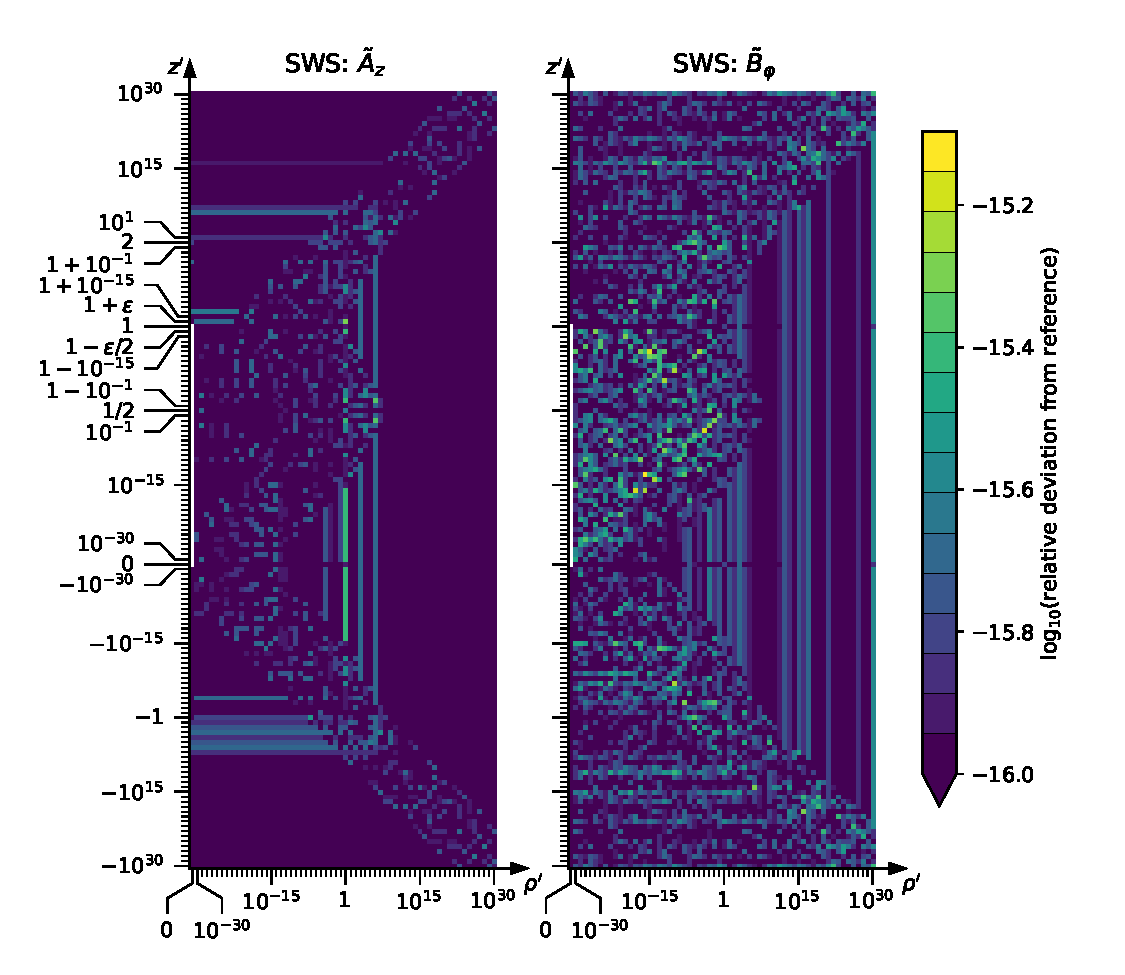
\includegraphics[width=\textwidth]{img/StraightWireSegment_results.pdf}
%  \includegraphics[width=\textwidth]{img/figure_11.pdf}
 \caption{Deviation between the Java implementation of the methods for $\tilde{A}_z$ (left)
          and $\tilde{B}_\varphi$ (right) of a straight wire segment (SWS).
          The left  plot shows the deviation between the Java implementation of \eqn{sws_A_z_switchover}
                         and the arbitray-precision implementation of \eqn{sws_A_z_ref}
          and
          the right plot shows the deviation between the Java implementation of \eqn{sws_B_phi_switchover}
                         and the arbitray-precision implementation of \eqn{sws_B_phi_ref}
          in the error metric given by~\eqn{error_metric}.}
 \label{fig:StraightWireSegment_results}
\end{figure}
It is observed that the relative error is less that $10^{-15}$ for all test points under consideration.

\subsection{Circular Wire Loop}
Next, the results of the verification of the circular wire loop methods are presented.
The normalized tangential component of the magnetic vector potential, $\tilde{A}_\varphi$,
and the normalized radial and vertical components of the magnetic field, $\tilde{B}_\rho$ and $\tilde{B}_z$,
of a circular wire loop have been evaluated using \eqn{A_phi_final}, \eqn{cwl_B_rho_switchover}
and \eqn{cwl_B_z_switchover}, respectively,
on all test points in $T_\mathrm{CWL}$ (see Sec.~\ref{sec:methods_verification}).
Fig.~(\ref{fig:CircularWireLoop_A_phi_Java}) shows the deviation
according to the error metric~\eqn{error_metric}
between the reference data computed for $\tilde{A}_\varphi$ using \eqn{A_phi_ref}
and the results from the \texttt{binary64} implementation of \eqn{A_phi_final}.
\begin{figure}[htbp]
 \centering
 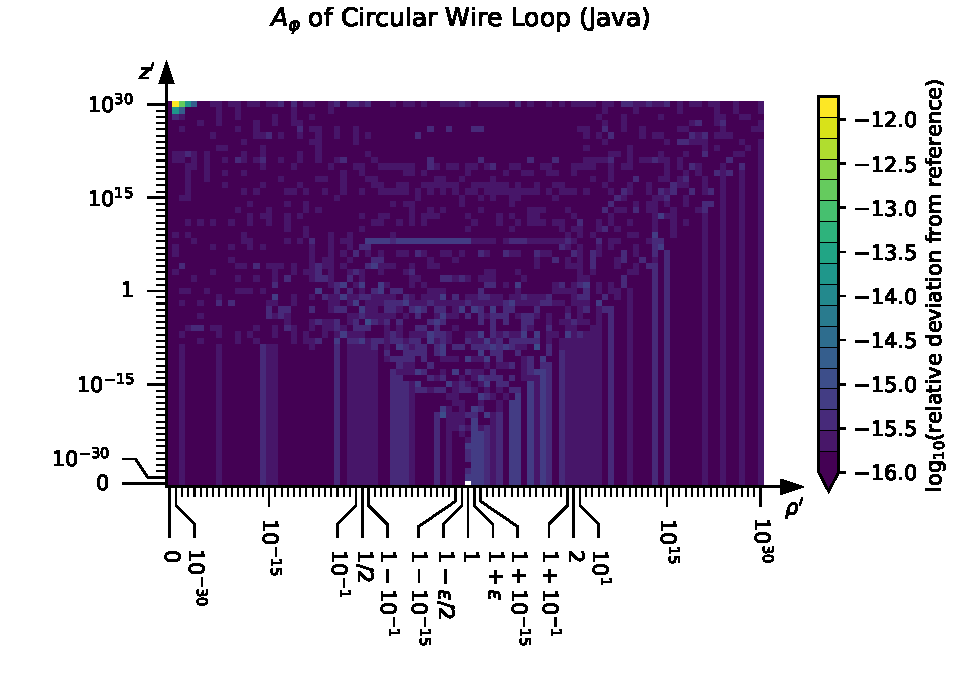
\includegraphics[width=0.8\textwidth]{img/CircularWireLoop_A_phi_Java.pdf}
%  \includegraphics[width=0.8\textwidth]{img/figure_12.pdf}
 \caption{Deviation between Java implementation of \eqn{A_phi_final} and \eqn{A_phi_ref}
          for the computation of $\tilde{A}_\varphi$ of a circular wire loop
          in the error metric given by~\eqn{error_metric}.}
 \label{fig:CircularWireLoop_A_phi_Java}
\end{figure}
Fig.~(\ref{fig:CircularWireLoop_B_rho_Java}) shows the deviation
according to the error metric~\eqn{error_metric}
between the reference data computed for $\tilde{B}_\rho$ using \eqn{B_rho_ref}
and the results from the \texttt{binary64} implementation of \eqn{cwl_B_rho_switchover}.
\begin{figure}[htbp]
 \centering
 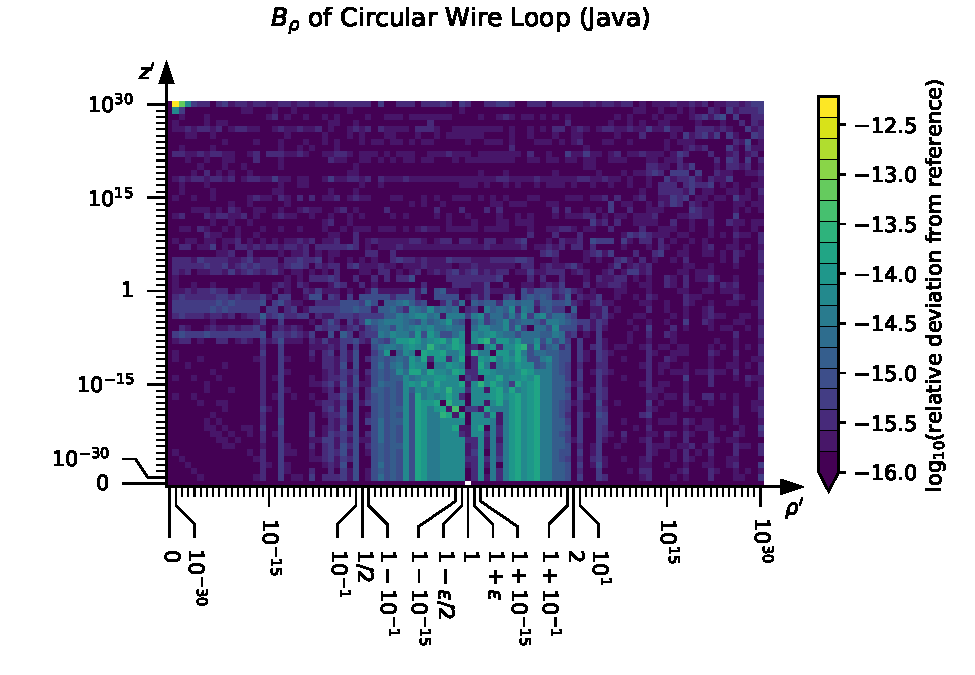
\includegraphics[width=0.8\textwidth]{img/CircularWireLoop_B_rho_Java.pdf}
%  \includegraphics[width=0.8\textwidth]{img/figure_13.pdf}
 \caption{Deviation between Java implementation of \eqn{cwl_B_rho_switchover} and \eqn{B_rho_ref}
          for the computation of $\tilde{B}_\rho$ of a circular wire loop
          in the error metric given by~\eqn{error_metric}.}
 \label{fig:CircularWireLoop_B_rho_Java}
\end{figure}
Fig.~(\ref{fig:CircularWireLoop_B_z_Java}) shows the deviation
according to the error metric~\eqn{error_metric}
between the reference data computed for $\tilde{B}_z$ using \eqn{B_z_ref}
and the results from the \texttt{binary64} implementation of \eqn{cwl_B_z_switchover}.
\begin{figure}[htbp]
 \centering
 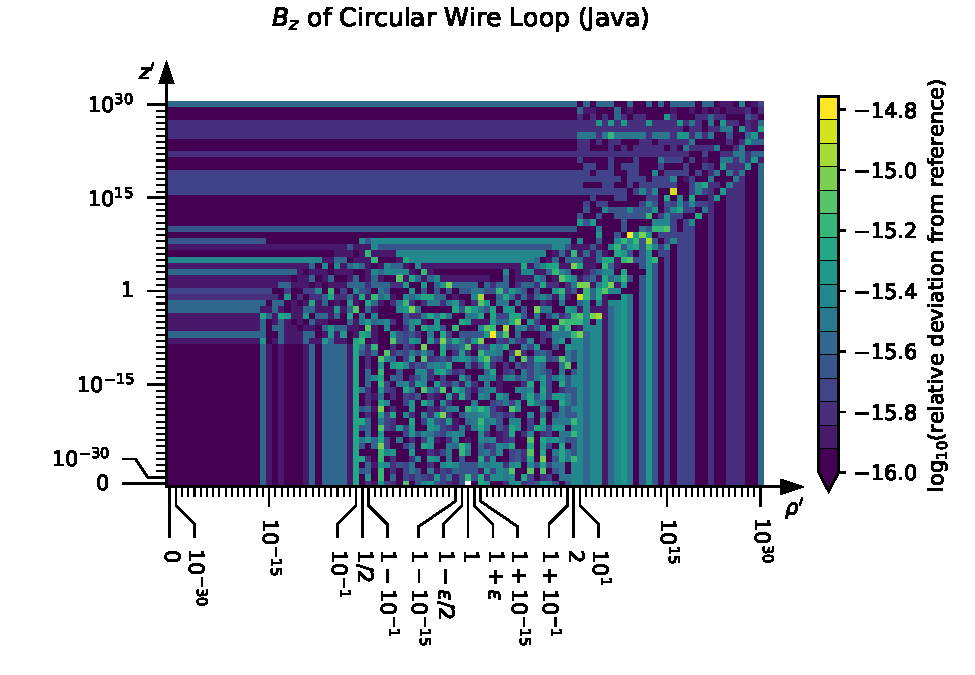
\includegraphics[width=0.8\textwidth]{img/CircularWireLoop_B_z_Java.pdf}
%  \includegraphics[width=0.8\textwidth]{img/figure_14.pdf}
 \caption{Deviation between Java implementation of \eqn{cwl_B_z_switchover} and \eqn{B_z_ref}
          for the computation of $\tilde{B}_z$ of a circular wire loop
          in the error metric given by~\eqn{error_metric}.}
 \label{fig:CircularWireLoop_B_z_Java}
\end{figure}

\FloatBarrier
\subsection{Further tests}
Furthermore, it was tested if the methods presented in this work
can be used to approximate a circular wire loop
by a polygon along the wire down to numerical accuracy.
The geometry of the setup is depicted in Fig.~(\ref{fig:sketch_McGreivy}).
\begin{figure}[htbp]
 \centering
 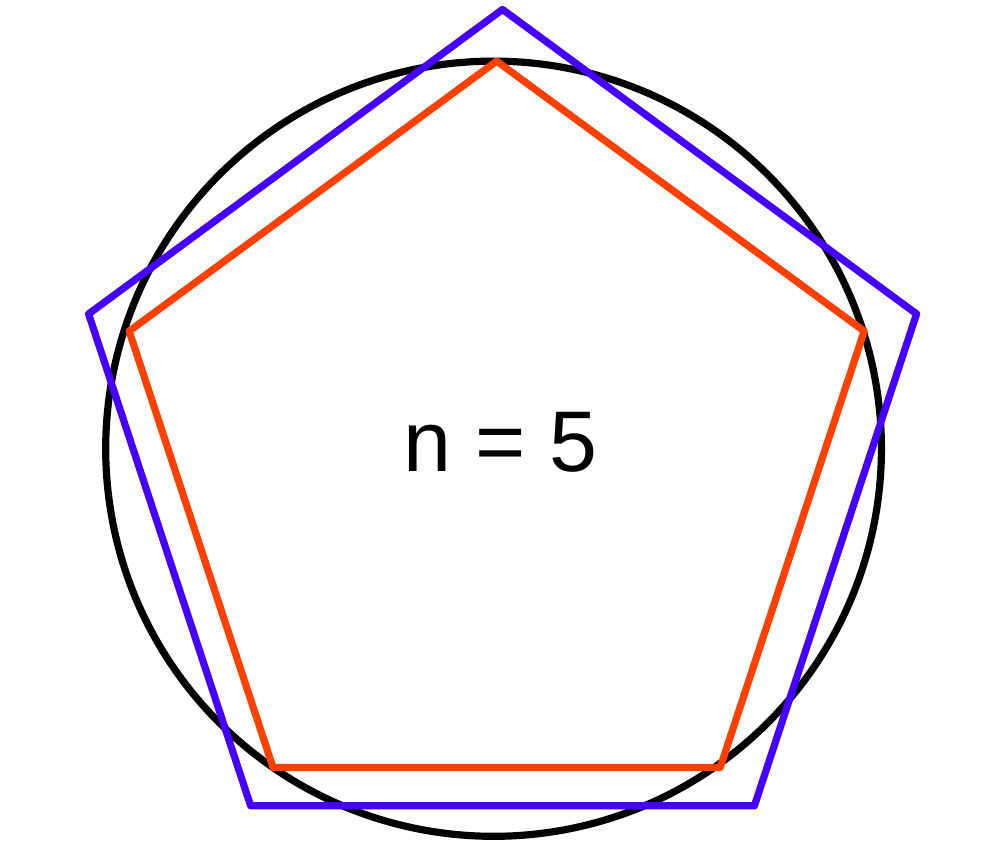
\includegraphics[width=0.4\textwidth]{img/sketch_McGreivy.png}
%  \includegraphics[width=0.4\textwidth]{img/figure_15.png}
 \caption{Sketch of the test setup for approximating a circular wire loop by a polygon.
          The current along the wire loop (black) is approximated by
          a current along a polygon with vertices either on the loop (red)
          or vertices adjusted slightly outwards (blue).
          The case of $n=5$ vertices used to approximate the loop is shown here.}
 \label{fig:sketch_McGreivy}
\end{figure}
The expected result is that the relative deviation between
the magnetic field at an arbitrary location
from the circular wire loop and from the corresponding polygon approximation
using straight wire segments vanishes down to numerical accuracy
for a sufficiently large number of points~$n$ used to approximate the wire loop.
A second-order correction to the polygon approximation
for a circular wire loop~\cite{mcgreivy_2021} can be used
to improve the approximation.
Here, the vertices of the polygon used to approximate the wire loop
are adjusted slightly outwards.
Figuratively speaking, in the default case (red polygon in Fig.~\ref{fig:sketch_McGreivy})
the polygon segments are always inside the wire loop
and in the adjusted case (blue polygon in Fig.~\ref{fig:sketch_McGreivy}),
the polygon segments have portions both inside and outside the wire loop.
The results of increasing the number of polygon corners
and observing the decay of the relative error between the analytical wire loop
expression and the approximation by the polygon
are shown in Fig.~(\ref{fig:McGreivy_convergence_2}),
where the orange graph with + symbols (``on-loop'') denotes the case of the polygon vertices on the loop
and the cyan graph with x symbols (``McGreivy'') denotes the case of the polygon vertices adjusted towards the outside
according to Ref.~\cite{mcgreivy_2021}.
In those two cases, standard accumulation using the \texttt{+=} operator
was used to sum up the contributions from the individual wire segments.
It is observed that the results approach numerical accuracy.
but then the error grows again if more polygon vertices are used for the approximation.
This can be explained by considering that the more vertices are used,
the smaller the relative contributions from each individual segment to the total approximation get.
If standard accumulation of the results is used, at some number of polygon corners
it happens that the remaining contributions are getting smaller than the machine precision epsilon
of the current approximation result, thereby effectively ignoring the remaining contributions.
Second-order iterative Kahan-Babuska summation~\cite{klein_2006} had to be used
to circumvent this and achieve convergence down to numerical accuracy.
This is shown by the red and blue graphs labeled ``K-B'' in Fig.~(\ref{fig:McGreivy_convergence_2}),
where the relative deviation from the reference data does not grow
as the number of polygon corners is increased beyond the threshold for an accurate approximation.
\begin{figure}[htbp]
 \centering
 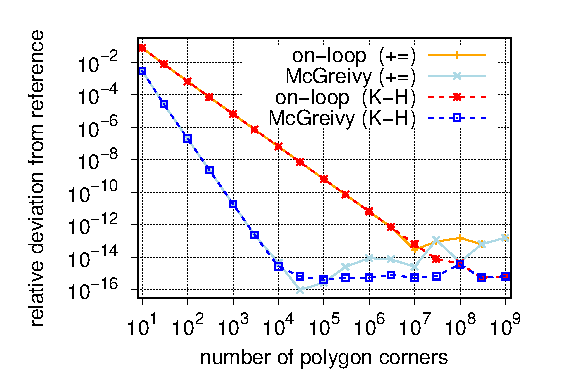
\includegraphics[width=0.8\textwidth]{img/McGreivy_convergence_2.eps}
%  \includegraphics[width=0.8\textwidth]{img/figure_16.eps}
 \caption{Convergence of the polygon approximation towards the analytical result for the magnetic field of a circular wire loop.
          The vertices of the polygon used to approximate the wire loop have been put on the wire loop (``on-loop'')
          as well as adjusted slightly outwards of the loop according to Ref.~\cite{mcgreivy_2021} (``McGreivy'').
          Standard accumulation using the \texttt{+=} operator (``+='') has been used for the first two graphs (orange and cyan).
          The second two graphs (red and blue) show the results when the accumulation of the individual contributions
          is performed using compensated Kahan-Babushka summation~\cite{klein_2006} (``K-B'').}
 \label{fig:McGreivy_convergence_2}
\end{figure}
